\documentclass[aspectratio=169,11pt]{beamer}

\usetheme{metropolis}

\usepackage{booktabs}
\usepackage{graphicx}
\usepackage{tikz}
\usepackage{appendixnumberbeamer}

% ── Colour palette ──────────────────────────
\definecolor{bg}{HTML}{33271E}
\definecolor{muted}{HTML}{8A7B94}
\definecolor{sage}{HTML}{8FBCB3}
\definecolor{lime}{HTML}{C8E88F}
\definecolor{cream}{HTML}{F6F4E8}

% ── Apply palette to beamer elements ────────
\setbeamercolor{normal text}{fg=cream, bg=bg}
\setbeamercolor{alerted text}{fg=lime}
\setbeamercolor{example text}{fg=sage}

\setbeamercolor{frametitle}{fg=cream, bg=bg}
\setbeamercolor{title}{fg=cream, bg=bg}
\setbeamercolor{subtitle}{fg=sage}
\setbeamercolor{author}{fg=cream}
\setbeamercolor{institute}{fg=muted}
\setbeamercolor{date}{fg=muted}

\setbeamercolor{progress bar}{fg=sage, bg=bg!80!black}
\setbeamercolor{title separator}{fg=sage}

\setbeamercolor{block title}{fg=bg, bg=sage}
\setbeamercolor{block body}{fg=cream, bg=bg!85!black}

\setbeamercolor{block title alerted}{fg=bg, bg=lime}
\setbeamercolor{block body alerted}{fg=cream, bg=bg!85!black}

\setbeamercolor{item}{fg=sage}
\setbeamercolor{subitem}{fg=muted}

\setbeamercolor{footnote}{fg=muted}
\setbeamercolor{footnote mark}{fg=muted}

\setbeamercolor{standout}{fg=bg, bg=sage}

% ── Fonts ───────────────────────────────────
\setbeamerfont{frametitle}{series=\bfseries}

% ── Custom command for question emphasis ────
\newcommand{\audience}[1]{%
  \vspace{0.5em}%
  {\color{lime}\textbf{Question:}} {\color{cream}#1}%
}

\title{Minerals, Markets, and Armed Conflict}
\subtitle{Critical Minerals in the Modern Green Economy}
\author{Elisa D'Amico \and P\"aivi Lujala}
\institute{University College Dublin \and University of Oulu}
\date{Milan Workshop, March 2025}

\begin{document}

\maketitle

% ═══════════════════════════════════════════════
% MOTIVATION
% ═══════════════════════════════════════════════

\begin{frame}{The Energy Transition Creates New Stakes}
\begin{itemize}
    \item The clean energy transition is reshaping global demand for minerals.
    \item Tantalum, tin, gallium, germanium, PGMs, cobalt\ldots{} all essential for batteries, semiconductors, and renewables.
    \item Africa holds substantial reserves of many of these minerals.
    \item The ``resource curse'' literature tells us mineral wealth can fuel violence. But does it have to?
\end{itemize}

\vspace{0.8em}
\textcolor{sage}{\textbf{Central question:}} Does governance structure determine whether mineral discovery leads to conflict or pacification?
\end{frame}

% ═══════════════════════════════════════════════
% FRAMEWORK
% ═══════════════════════════════════════════════

\begin{frame}{The Governance--Value Nexus}
We propose three pathways from mineral discovery to conflict, distinguished by governance regime:

\vspace{0.8em}
\begin{columns}[T]
\column{0.32\textwidth}
\centering
\textcolor{sage}{\textbf{International Governance}}\\[4pt]
{\small Tantalum, Tin (3T)}\\[4pt]
{\footnotesize Dodd--Frank \S1502, iTSCi, OECD guidelines}\\[6pt]
{\footnotesize $\downarrow$ Revenue to armed groups\\$\downarrow$ Conflict events \textbf{and} deaths}

\column{0.32\textwidth}
\centering
\textcolor{lime}{\textbf{Governance Gap}}\\[4pt]
{\small Gallium, Germanium}\\[4pt]
{\footnotesize No international/national framework}\\[6pt]
{\footnotesize $\downarrow$ Conflict events\\$\uparrow$ Deaths \textit{when} violence occurs}

\column{0.32\textwidth}
\centering
\textcolor{muted}{\textbf{National Governance}}\\[4pt]
{\small Platinum Group Metals}\\[4pt]
{\footnotesize SA's MPRDA, Mining Charter}\\[6pt]
{\footnotesize $\downarrow$ Non--state violence\\\textit{No effect} on deaths}
\end{columns}
\end{frame}

\begin{frame}{Hypotheses}
\begin{description}
    \item[\textcolor{sage}{H1}] \textcolor{sage}{International governance} (tantalum, tin): Discovery reduces \textbf{both} non--state violence events and battle deaths.
    \vspace{0.4em}
    \item[\textcolor{lime}{H2}] \textcolor{lime}{Governance gap} (gallium, germanium): Discovery reduces events but \textbf{increases} battle deaths conditional on conflict.
    \vspace{0.4em}
    \item[\textcolor{muted}{H3}] \textcolor{muted}{National governance} (PGMs): Discovery reduces non--state violence through state monopoly control, with \textbf{no effect} on deaths.
\end{description}
\end{frame}

% ═══════════════════════════════════════════════
% DATA AND METHODS
% ═══════════════════════════════════════════════

\begin{frame}{Data}
\begin{itemize}
    \item \textcolor{sage}{\textbf{Mineral discoveries:}} S\&P Global Market Intelligence (geocoded across Africa)
    \item \textcolor{sage}{\textbf{Conflict:}} UCDP--GED (event--level, with fatalities). Disaggregated by violence type: state--based, non--state, one--sided
    \item \textcolor{sage}{\textbf{Outcomes:}} (1) Non--state violence event counts* (2) Battle deaths (UCDP ``best'' estimate)
    \item \textcolor{sage}{\textbf{Unit of analysis:}} Hexagonal grid cells at 7 resolutions (25--300km). Main results at 100km
\end{itemize}
\end{frame}

\begin{frame}{Spatial Coverage}
\begin{center}
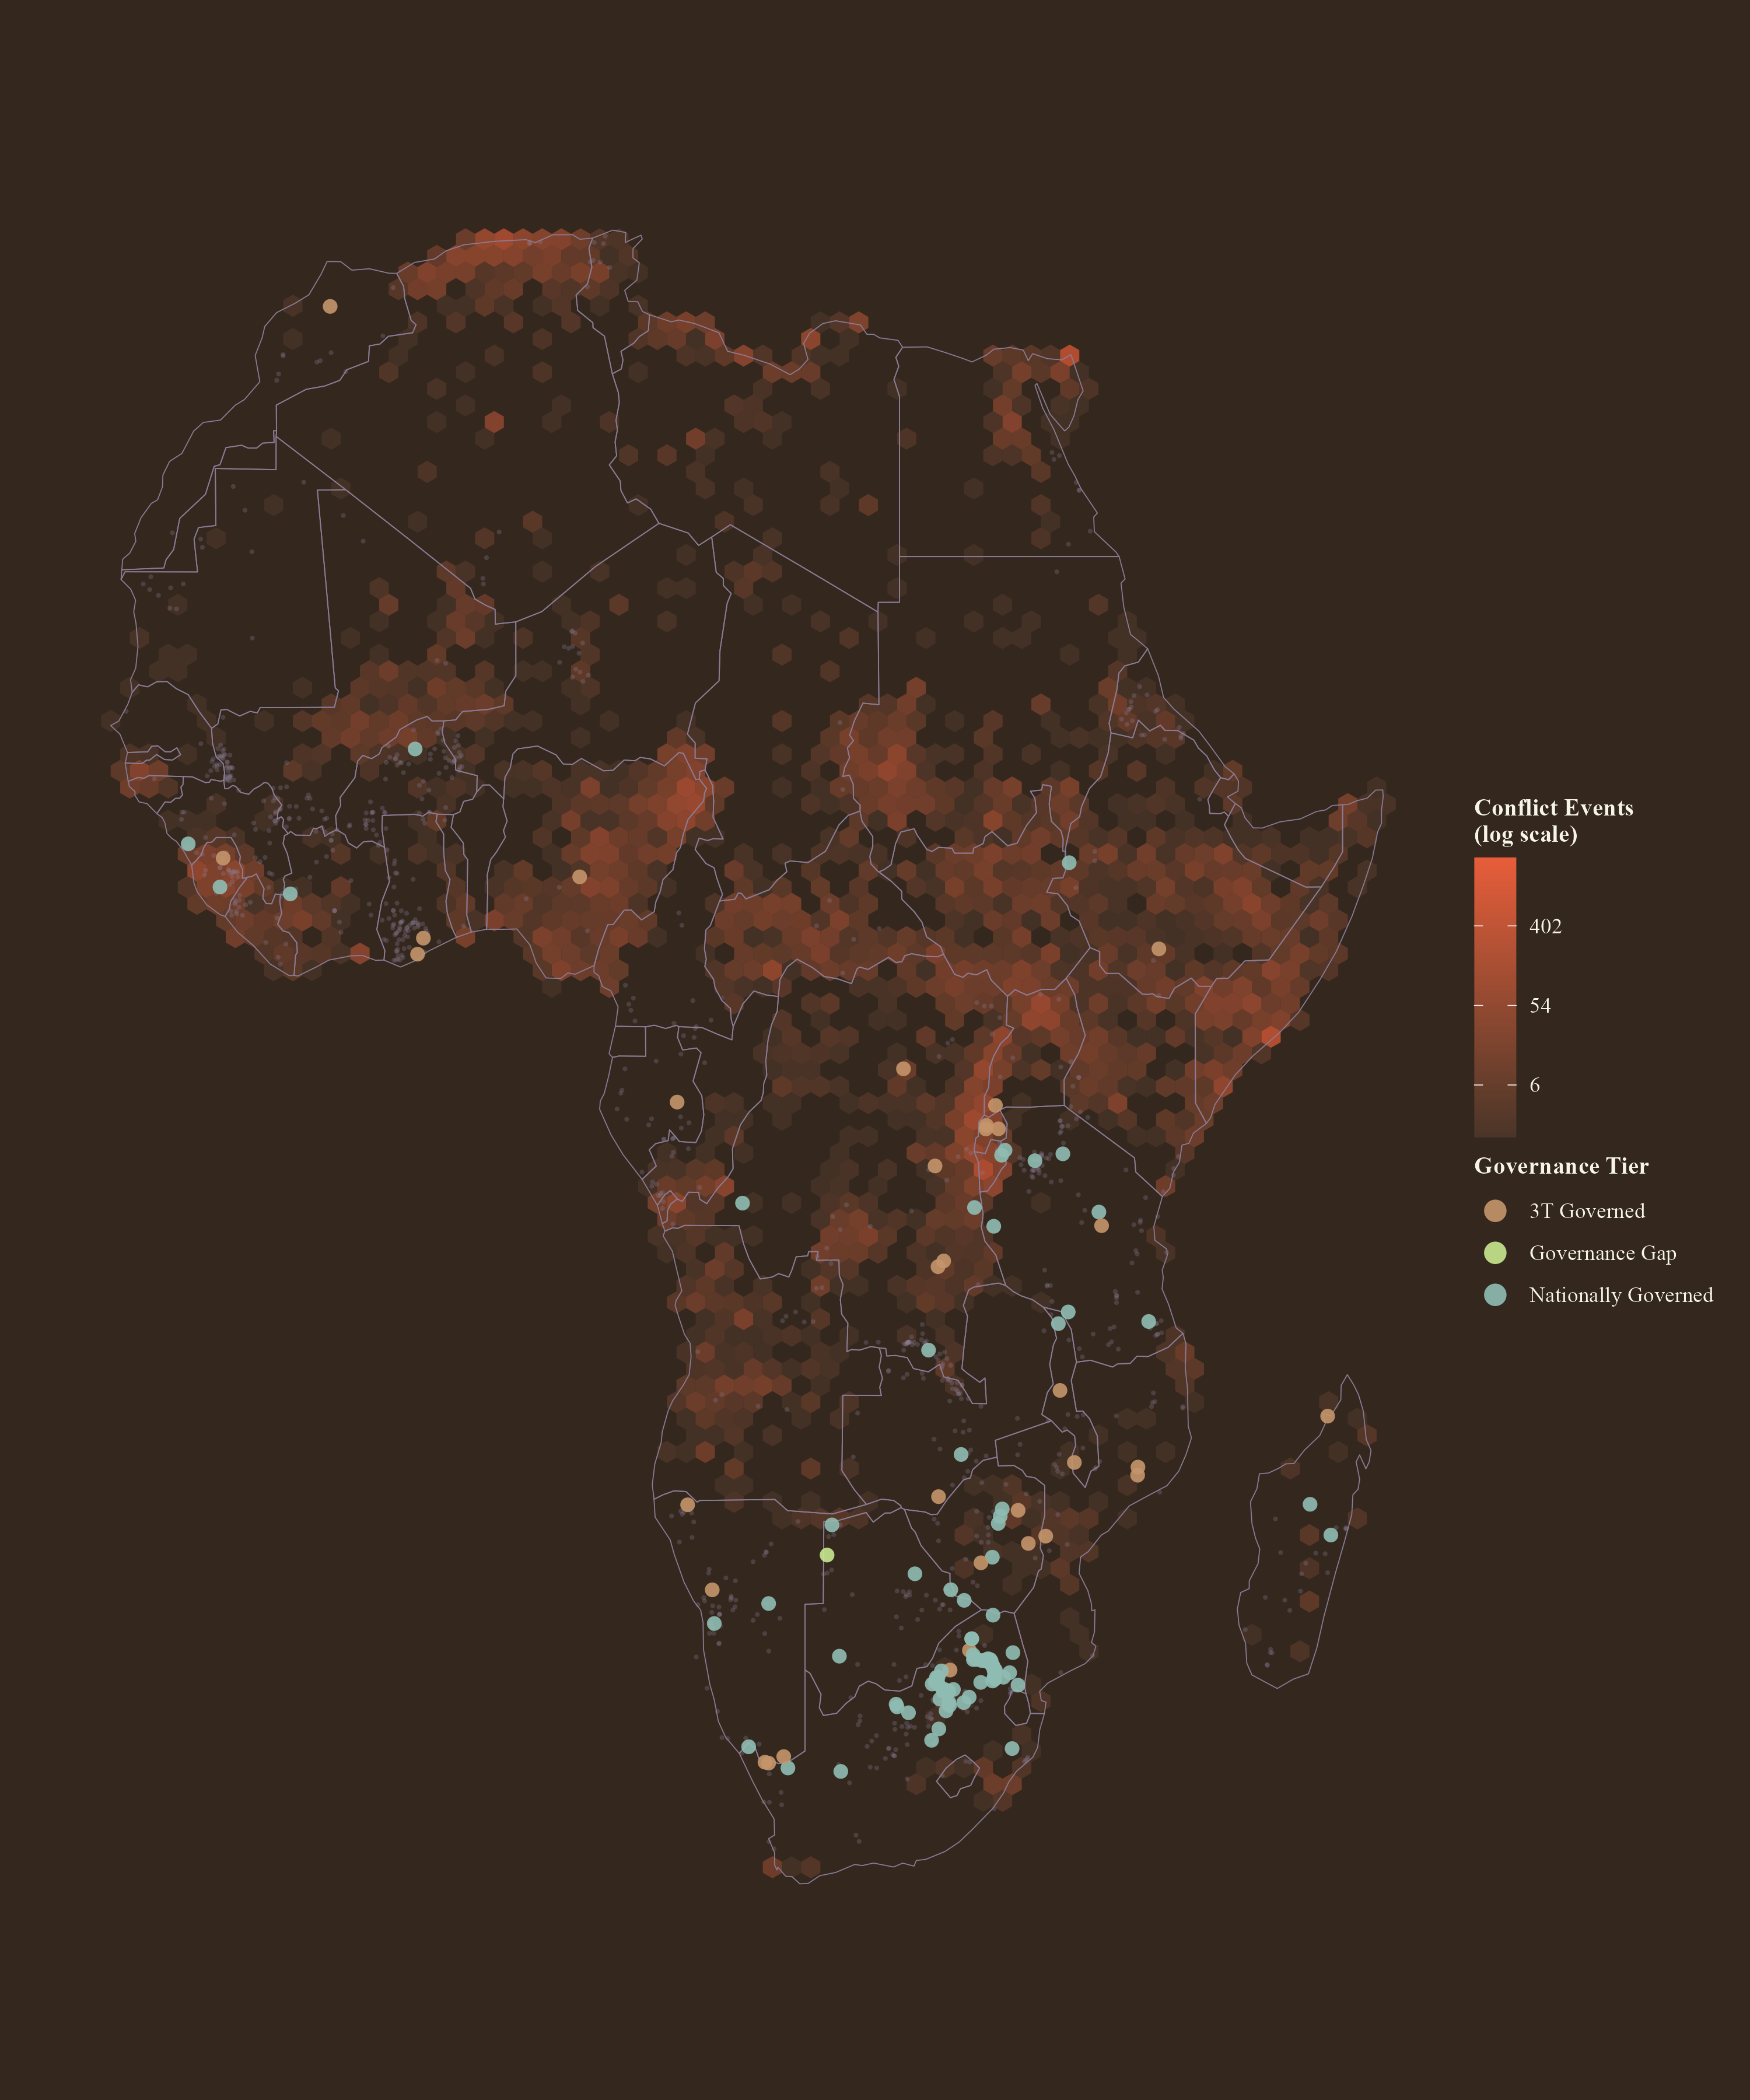
\includegraphics[
  width=0.5\textwidth,
  trim=0cm 3cm 0cm 3.5cm,
  clip
]{plots/africa_mineral_conflict_map.png}
\end{center}
\end{frame}

\begin{frame}{Empirical Strategy}
\begin{columns}[T]
\column{0.48\textwidth}
\vspace{0.3em}
{\small
\begin{itemize}
    \item Staggered DiD (Callaway \& Sant'Anna, 2021)
    \item Treatment: First mineral discovery in a grid cell
    \item Control Group: Not yet and never treated units
    \item Identifying Assumption: parallel trends
    \item Wild bootstrapped standard errors (clustering at cell level)
\end{itemize}
}
\column{0.50\textwidth}
\vspace{1.2em}
{\small Main specification:}
\vspace{0.3em}

{\footnotesize
\[
\text{Conflict}_{it} = \alpha_i + \lambda_t + \sum_{k=-K}^{K} \beta_k \cdot \text{Disc}_{it}^{k} + \varepsilon_{it}
\]
}

\vspace{0.5em}
{\footnotesize
\begin{tabular}{ll}
$\alpha_i$          & cell fixed effects \\
$\lambda_t$         & year fixed effects \\
$\text{Disc}_{it}^k$ & periods from discovery \\
$\beta_k$           & dynamic ATT ($k \geq 0$ post) \\
\end{tabular}
}
\end{columns}
\end{frame}

% ═══════════════════════════════════════════════
% RESULTS
% ═══════════════════════════════════════════════

\begin{frame}{\textcolor{sage}{H1: Tantalum} {\normalsize\color{muted}(3T Governed)}}
\begin{columns}[T]
\column{0.43\textwidth}
\vspace{0.5em}
{\small
\begin{itemize}
    \item Non--state violence declines significantly post--discovery and effects persist and strengthen.
    \item Battle deaths show modest decline in later periods.
    \item \textcolor{sage}{``Pure pacification.''} Consistent with international governance disrupting armed group financing.
\end{itemize}
}
\column{0.55\textwidth}
\centering
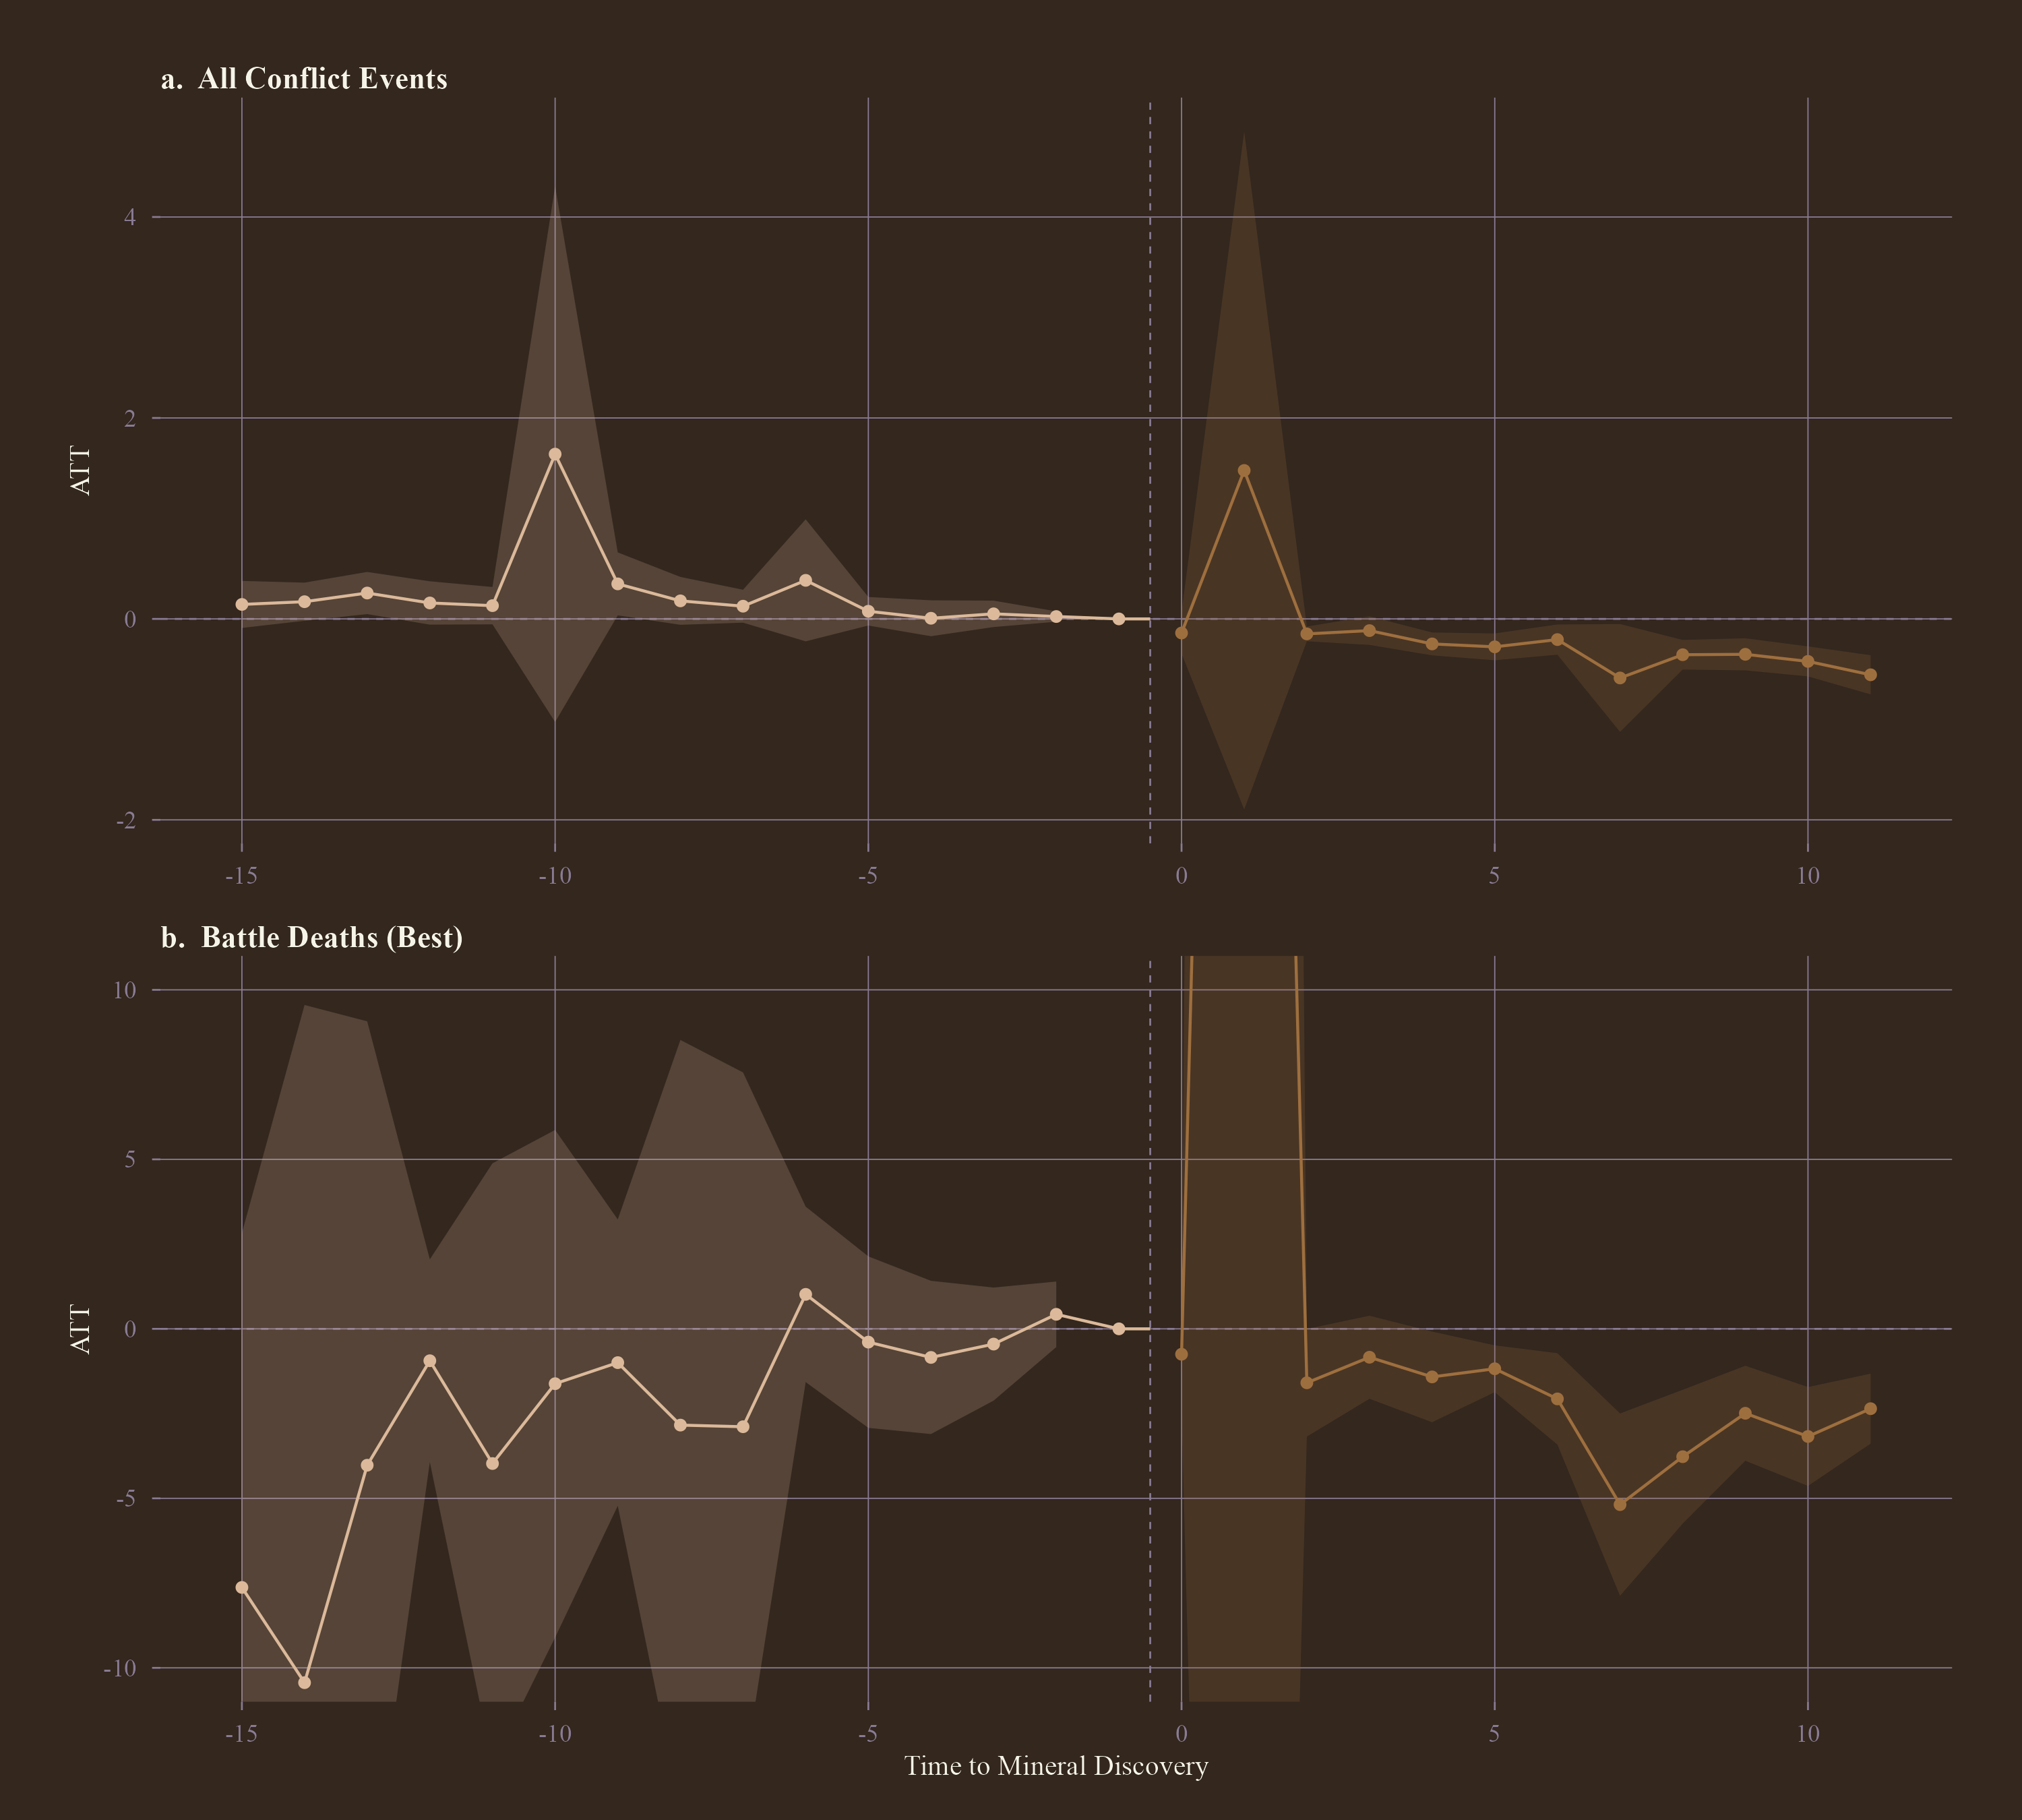
\includegraphics[width=\textwidth]{plots/tantalum_paired_event_study.png}
\end{columns}
\end{frame}

\begin{frame}{\textcolor{lime}{H2: Gallium \& Germanium} {\normalsize\color{muted}(Governance Gap)}}
\begin{columns}[T]
\column{0.43\textwidth}
\vspace{0.5em}
{\small
\begin{itemize}
    \item Non--state violence events decline (similar to governed minerals).
    \item But battle deaths \textbf{increase}. 
    \item \textcolor{lime}{``Decoupling.''} Fewer events, deadlier outcomes.
    \item Formalization may reduce petty violence while high strategic value attracts more capable actors.
\end{itemize}
}
\column{0.55\textwidth}
\centering
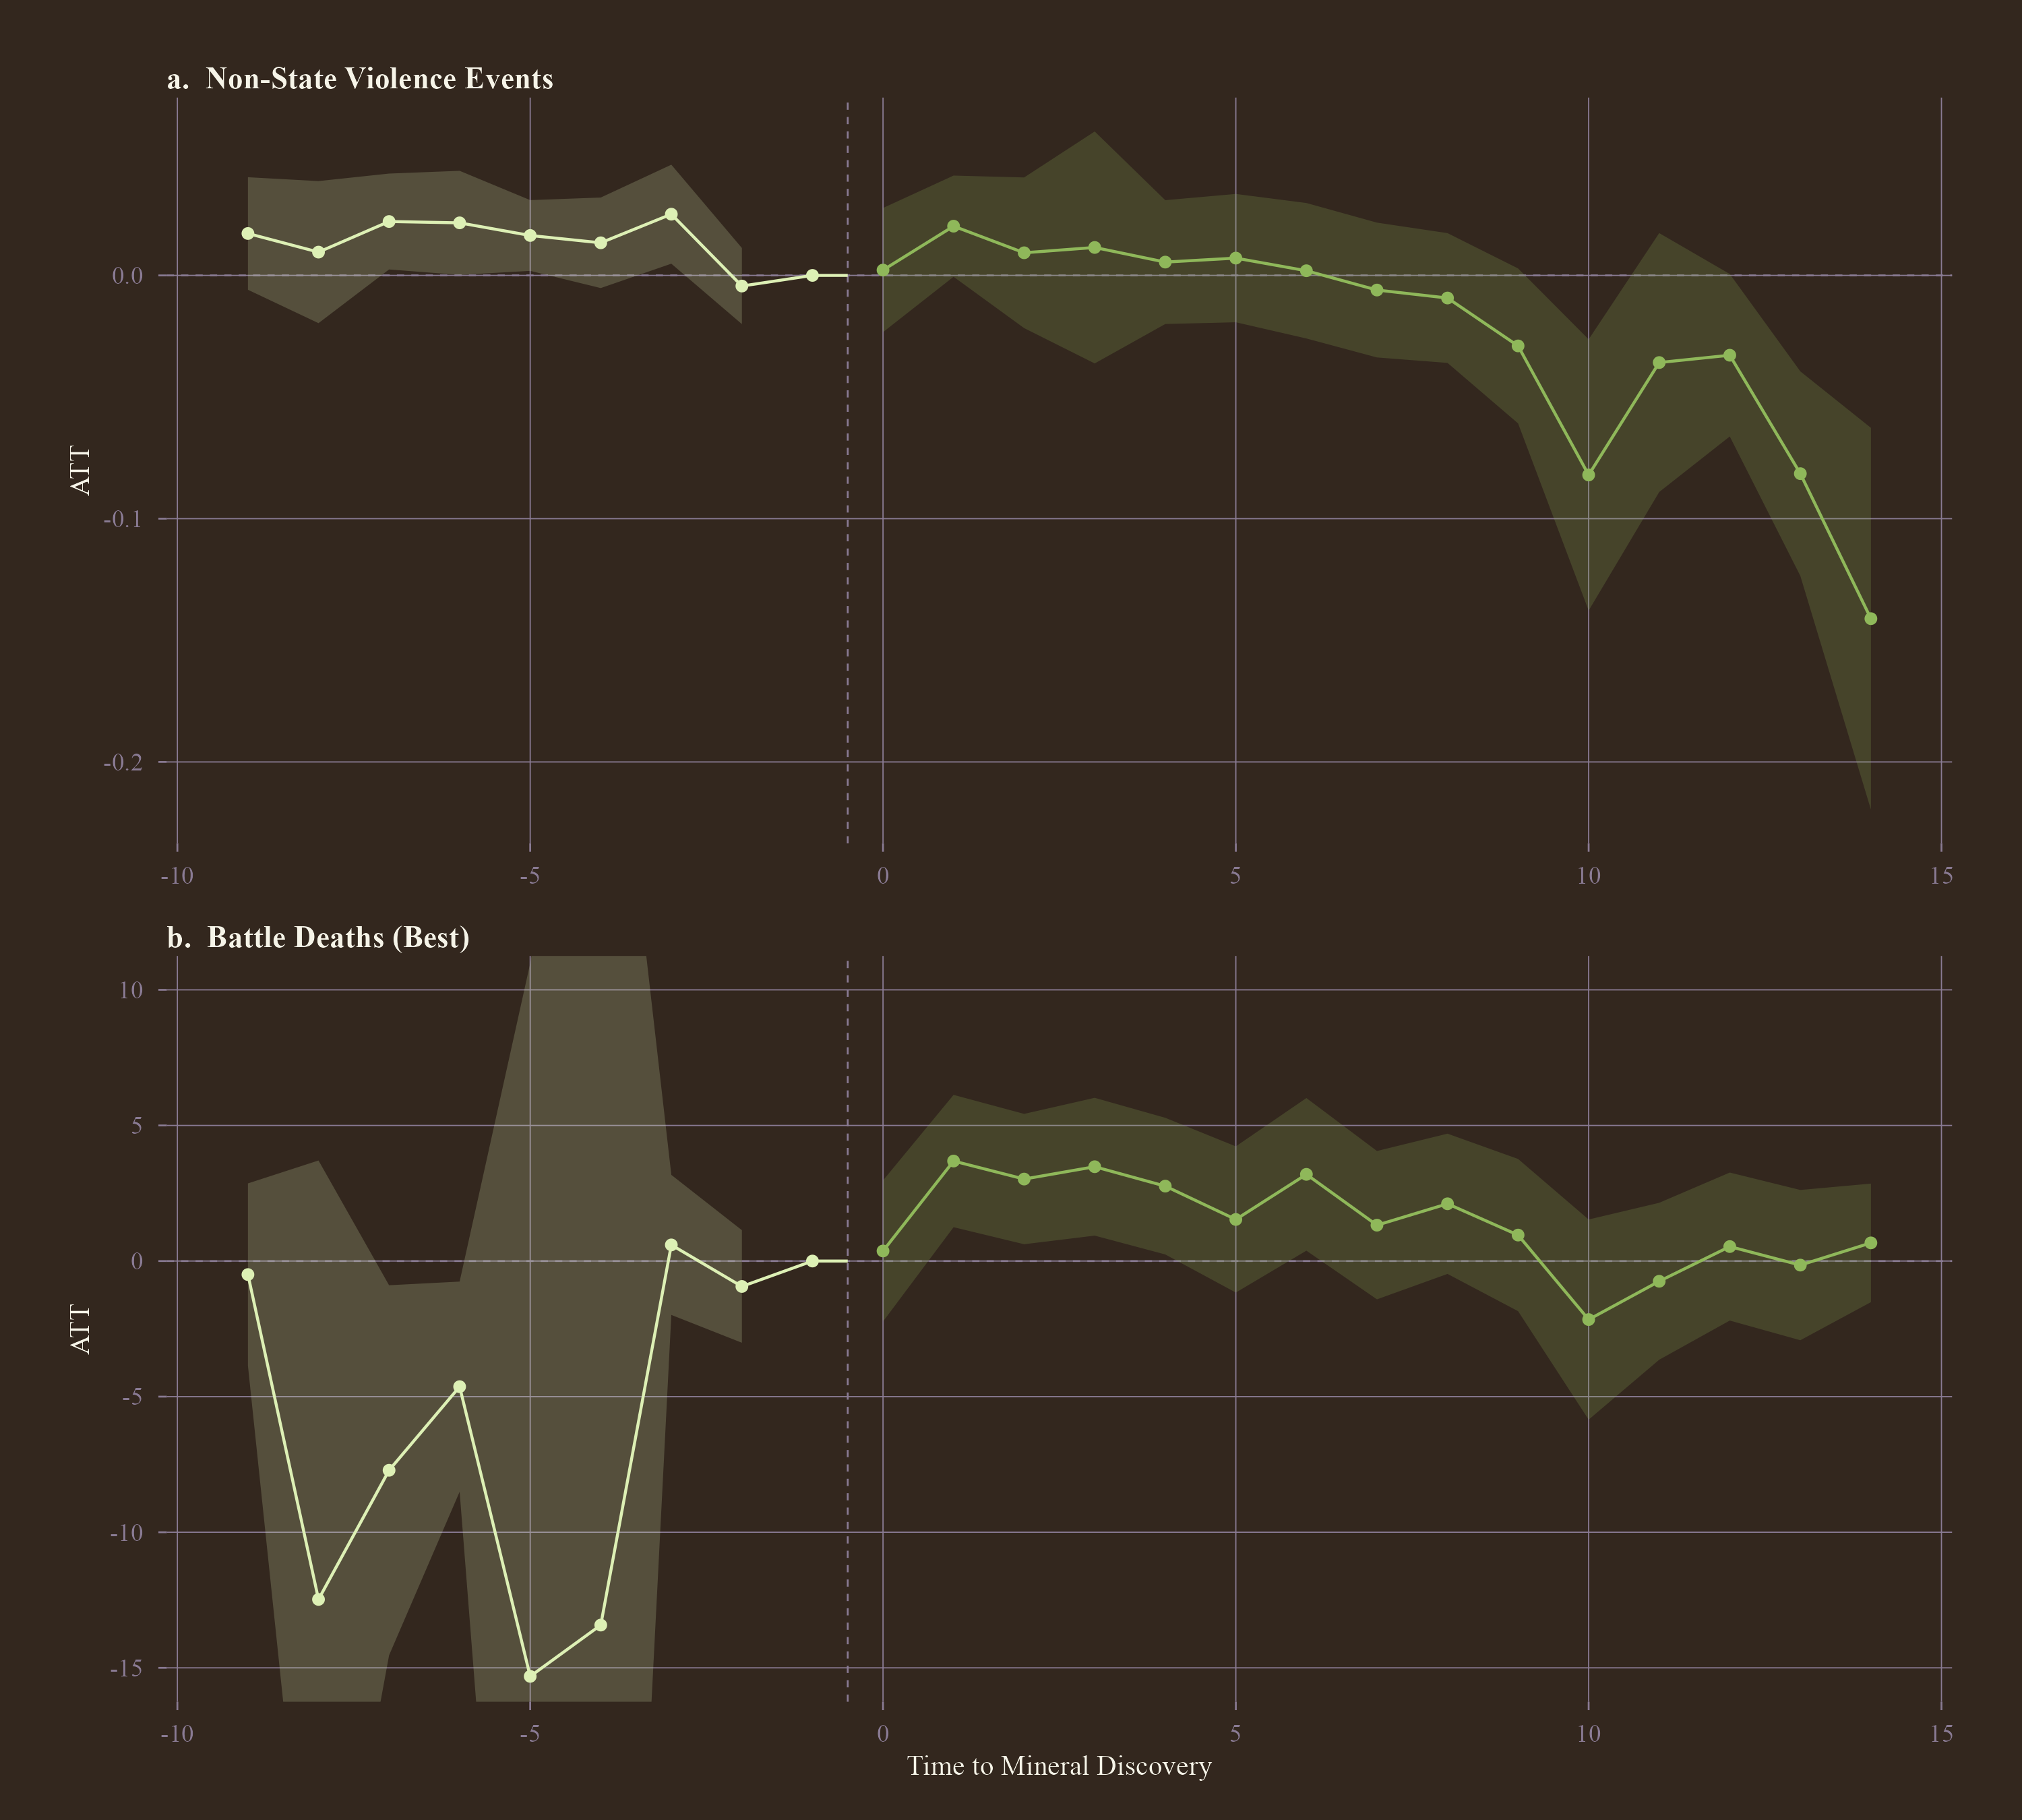
\includegraphics[width=\textwidth]{plots/gallium_germanium_paired_event_study.png}
\end{columns}
\end{frame}

\begin{frame}{\textcolor{muted}{H3: Platinum Group Metals} {\normalsize\color{muted}(Nationally Governed)}}
\begin{columns}[T]
\column{0.43\textwidth}
\vspace{0.5em}
{\small
\begin{itemize}
    \item Most consistent reduction in non--state violence of any mineral examined.
    \item Battle deaths: positive  but not statistically significant.
    \item Consistent with state monopoly control excluding armed groups from extraction.
\end{itemize}
}
\column{0.55\textwidth}
\centering
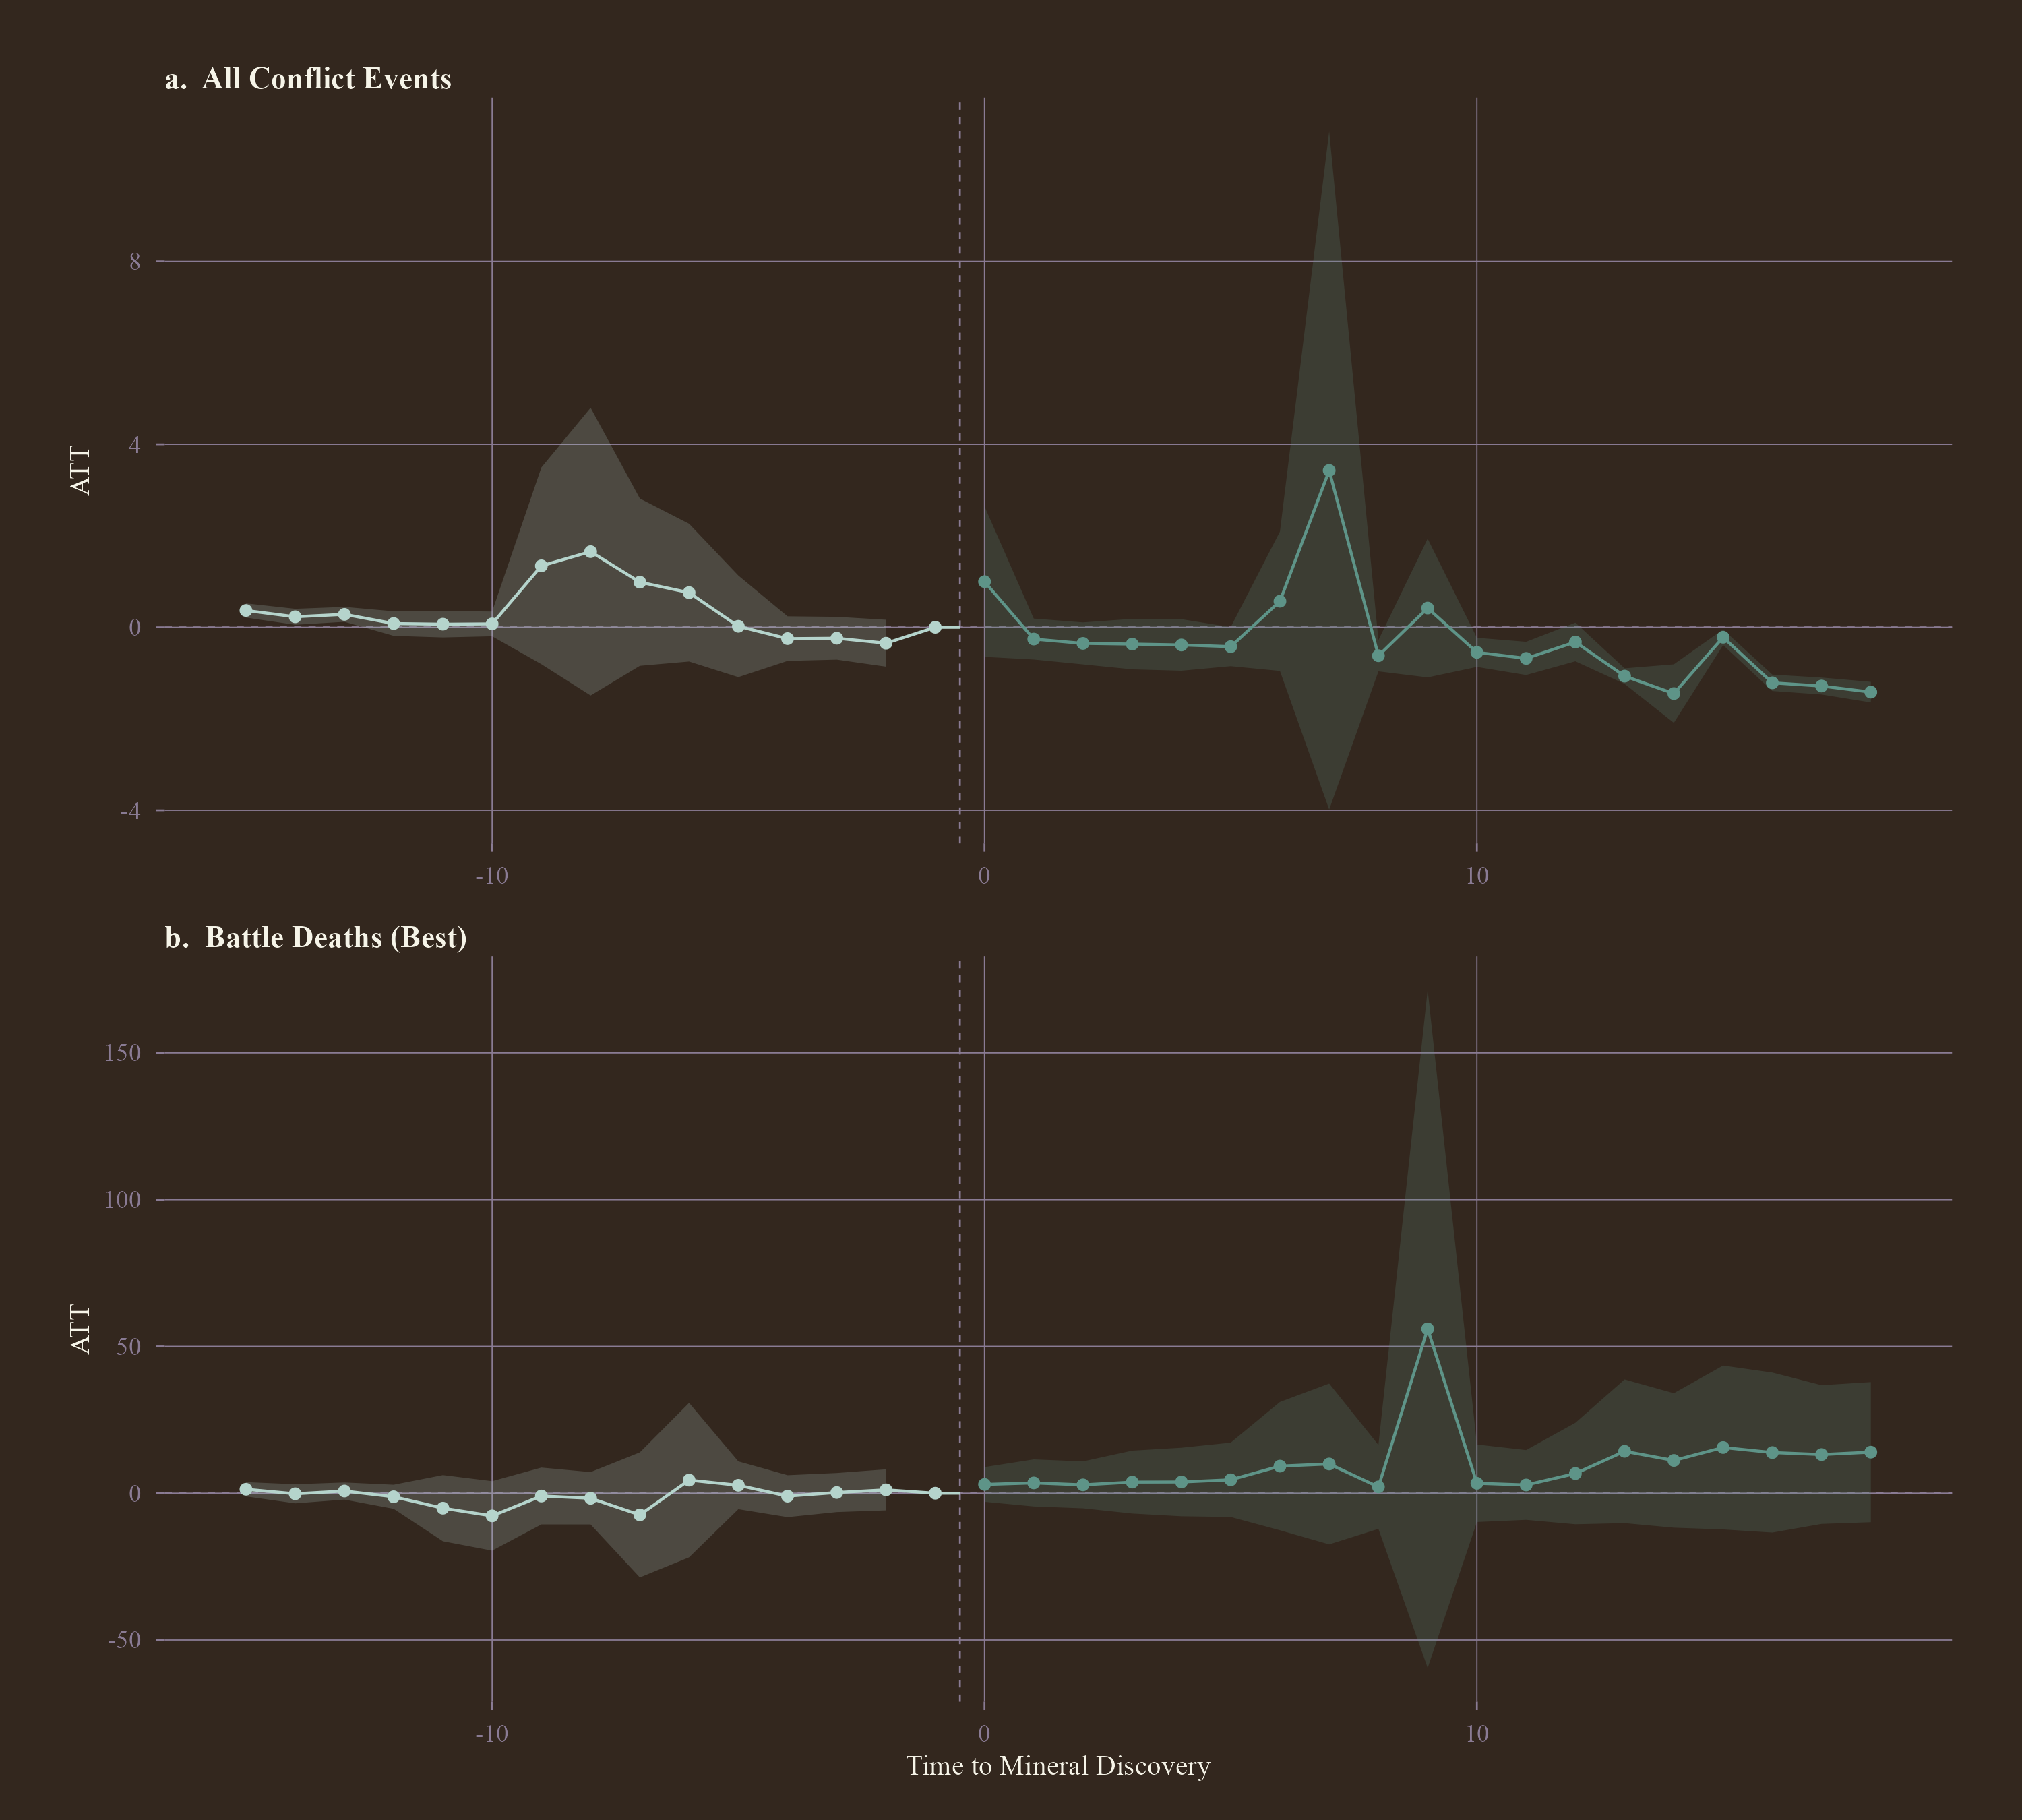
\includegraphics[width=\textwidth]{plots/pgms_paired_event_study.png}
\end{columns}
\end{frame}


\begin{frame}{Pooled Effects}
\begin{center}
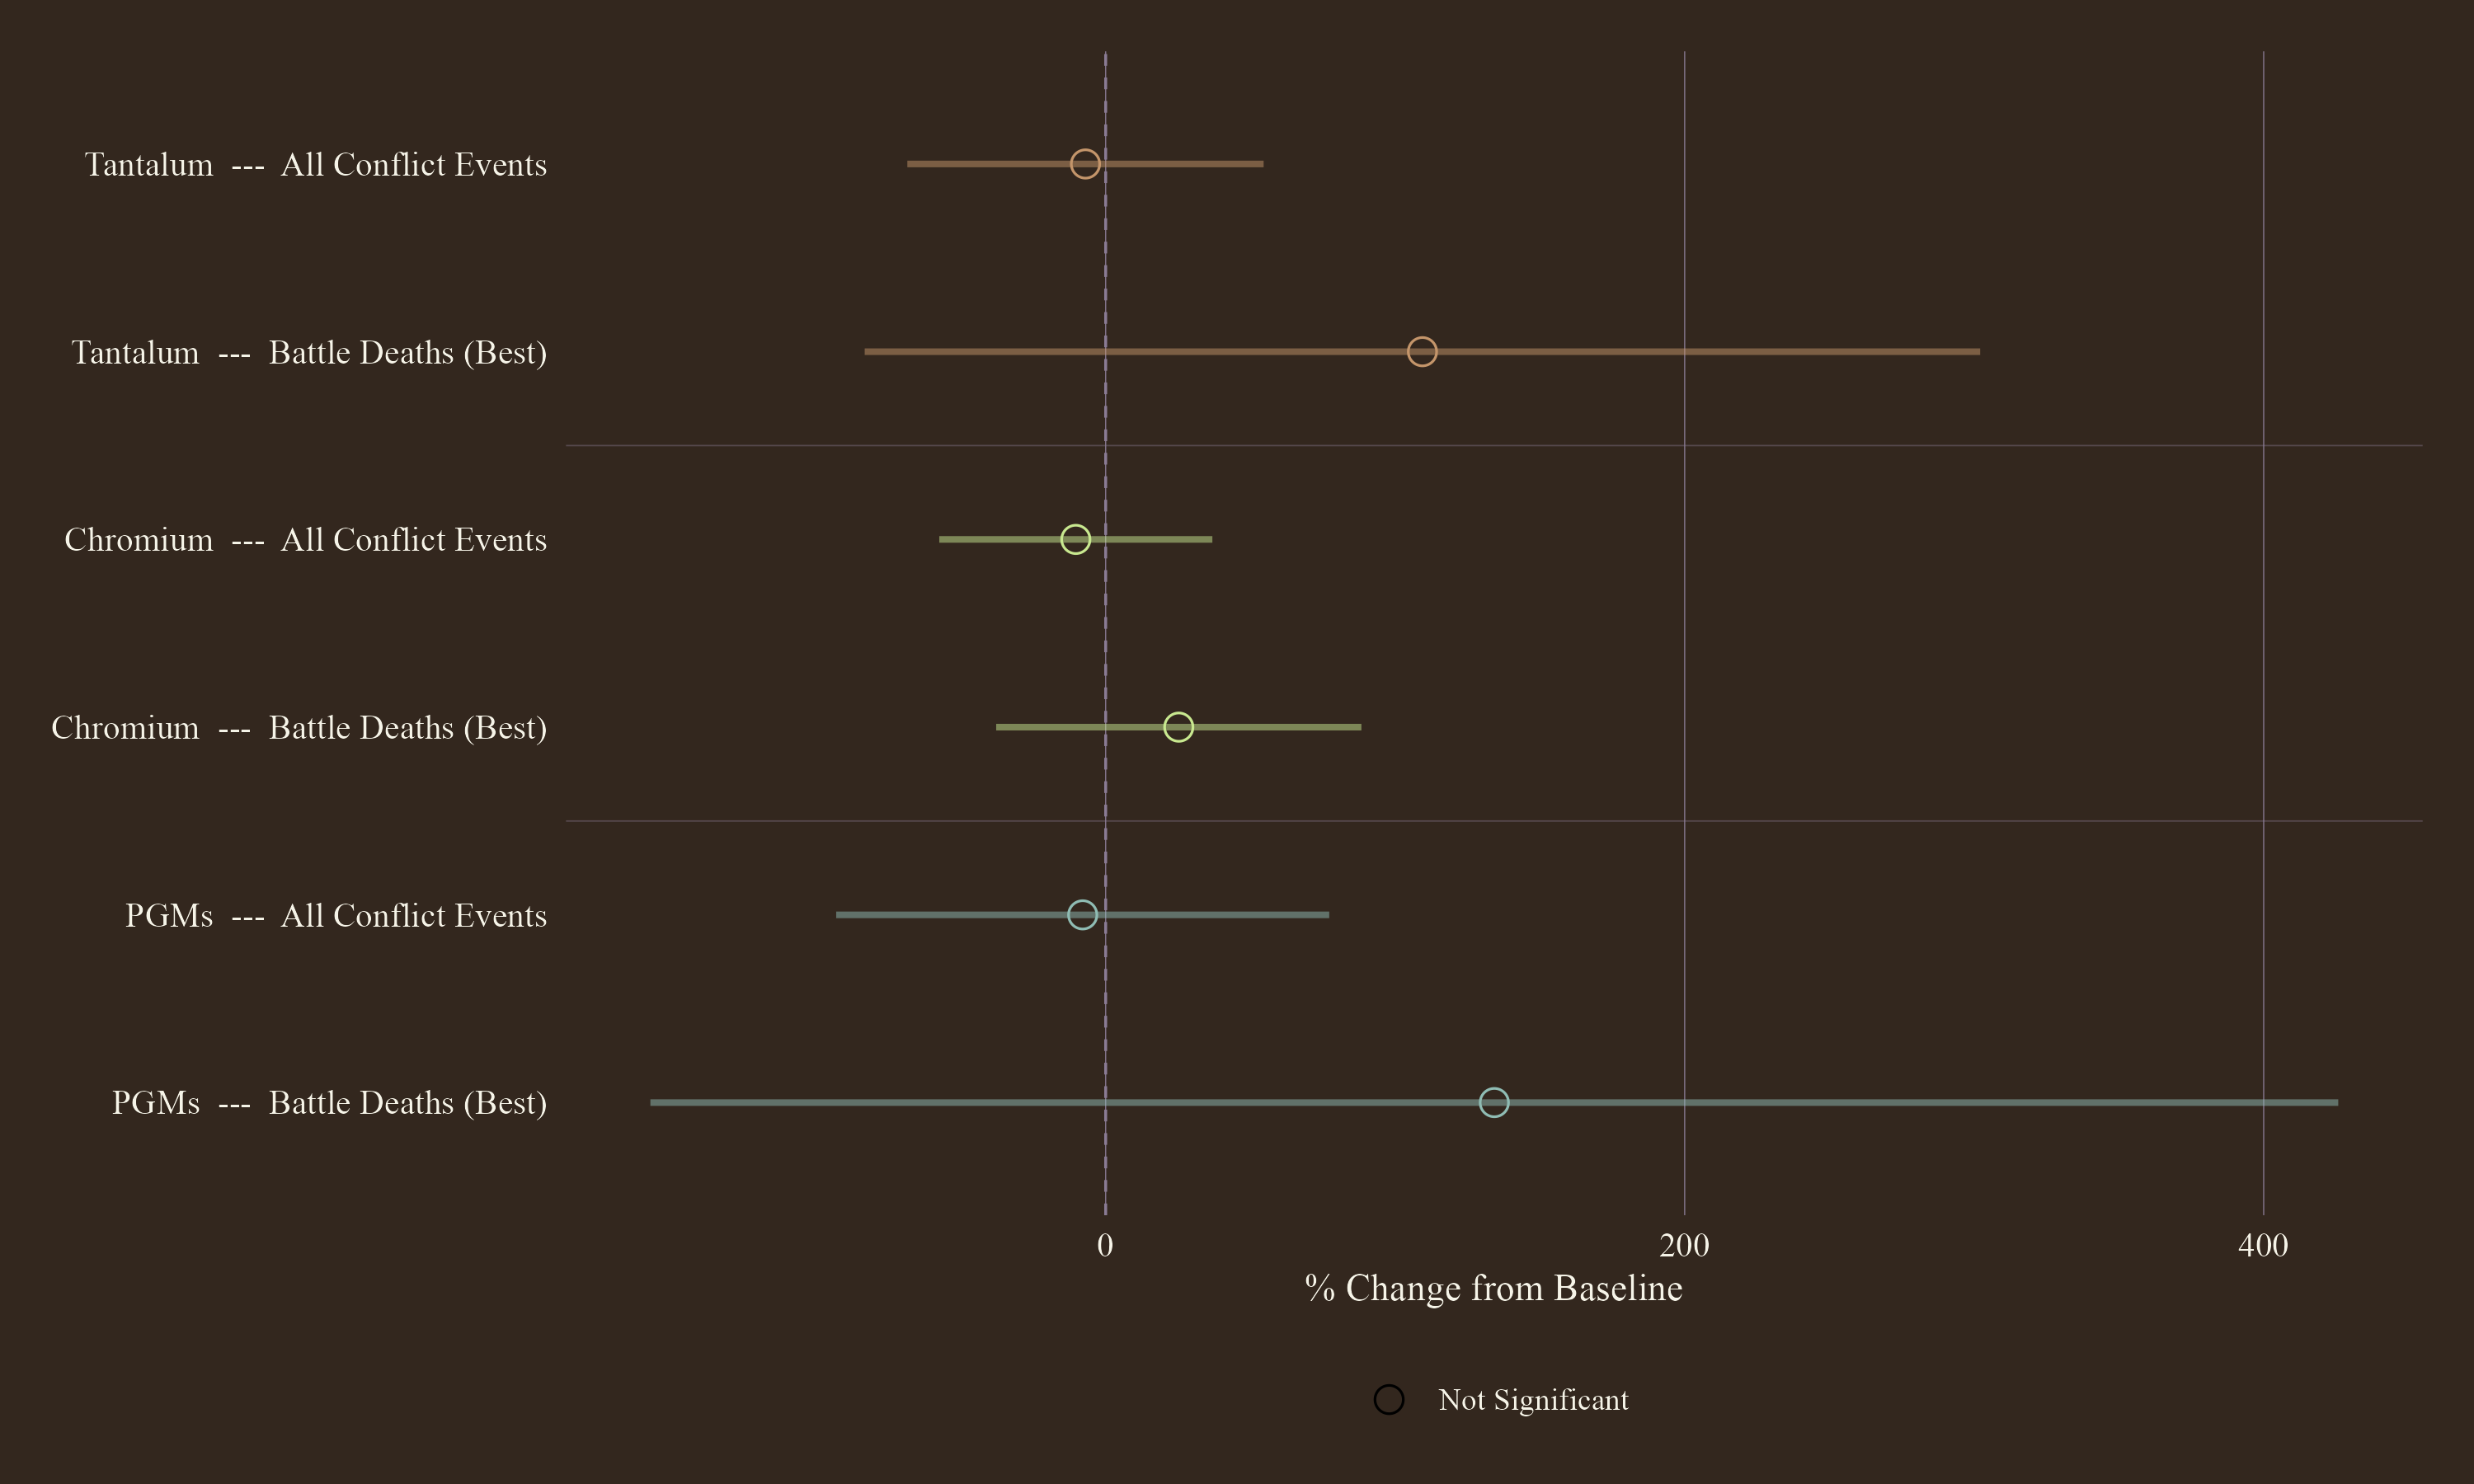
\includegraphics[width=0.65\textwidth]{plots/pooled_effects.png}
\end{center}

\vspace{-1.2em}
{\small
\begin{itemize}
    \item All three tiers reduce non--state violence: tantalum ($-77\%$), Ga/Ge ($-39\%$), PGMs ($-67\%$).
    \item Battle death effects null and positive (high variance in fatality counts).
\end{itemize}
}
\end{frame}

\begin{frame}{Calendar--Time Alignment with Policy Milestones}
\begin{columns}[T]
\column{0.45\textwidth}
\vspace{0.5em}
{\small
\begin{itemize}
    \item All three minerals trend downward together from $\sim$2012.
    \item \textcolor{lime}{Problem:} hard to distinguish governance effects from a common confound (e.g. peacekeeping expansion, economic development).
    \item \textit{Consistent with} the governance story, but cannot prove it.
\end{itemize}
}
\column{0.45\textwidth}
\centering
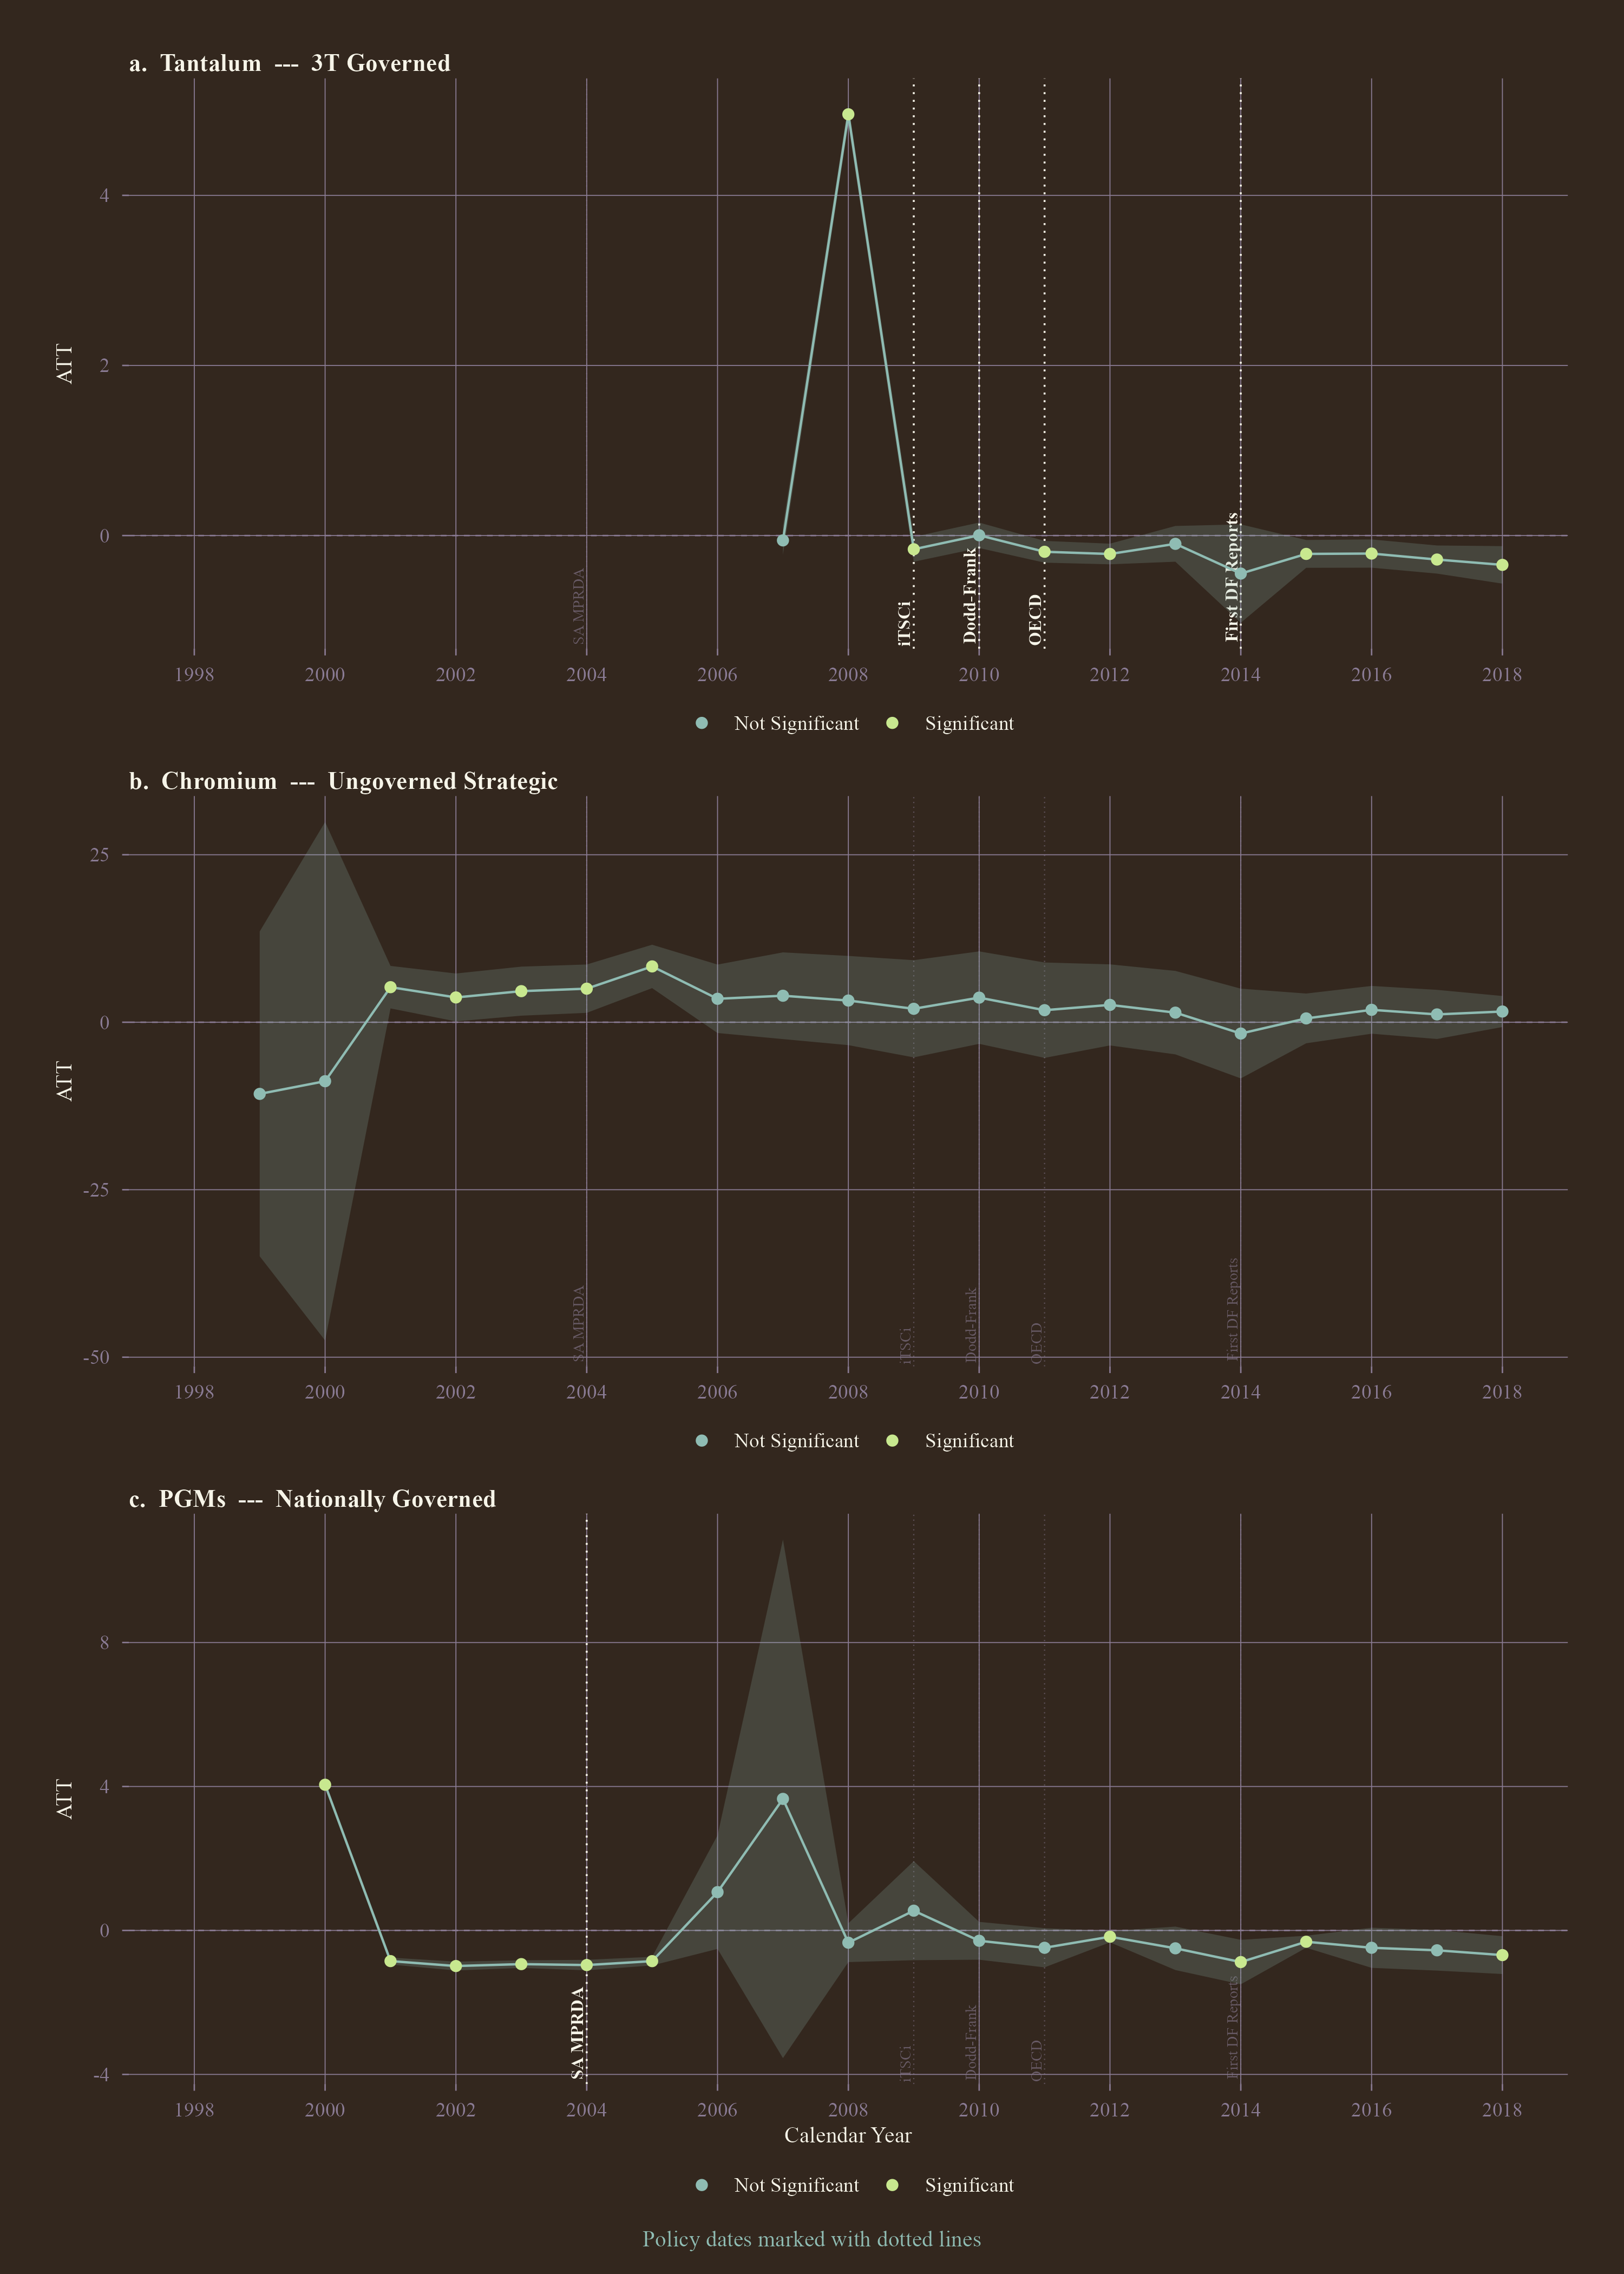
\includegraphics[width=\textwidth]{plots/all_minerals_calendar_comparison.png}
\end{columns}
\end{frame}


\begin{frame}{Spatial Scale Sensitivity}
\begin{columns}[T]
\column{0.45\textwidth}
\vspace{0.5em}
{\small
\begin{itemize}
    \item 3T minerals pacify at coarser scales, consistent with supply chain governance restructuring regional markets.
    \item Ga/Ge effects sharpen at fine scales. Without international frameworks, violence concentrates at extraction sites.
    \item PGM stability across all resolutions reflects formal state institutions whose reach does not attenuate with distance.
\end{itemize}
}
\column{0.53\textwidth}
\vspace{2.9em}
{\footnotesize
\begin{tabular}{llc}
\toprule
\textcolor{sage}{\textbf{Mineral}} & \textcolor{sage}{\textbf{Strongest Scale}} & \textcolor{sage}{\textbf{Decoup.}} \\
\midrule
Tantalum   & 250km (regional)   & No  \\
Tin        & 200--250km          & No  \\
Ga/Ge      & 25--50km (local)   & Yes \\
PGMs       & Stable (all)       & No  \\
\bottomrule
\end{tabular}

\vspace{0.8em}
}
\end{columns}
\end{frame}

\begin{frame}{Spatial Grid Structure}
\begin{columns}[T]
\column{0.39\textwidth}
\centering
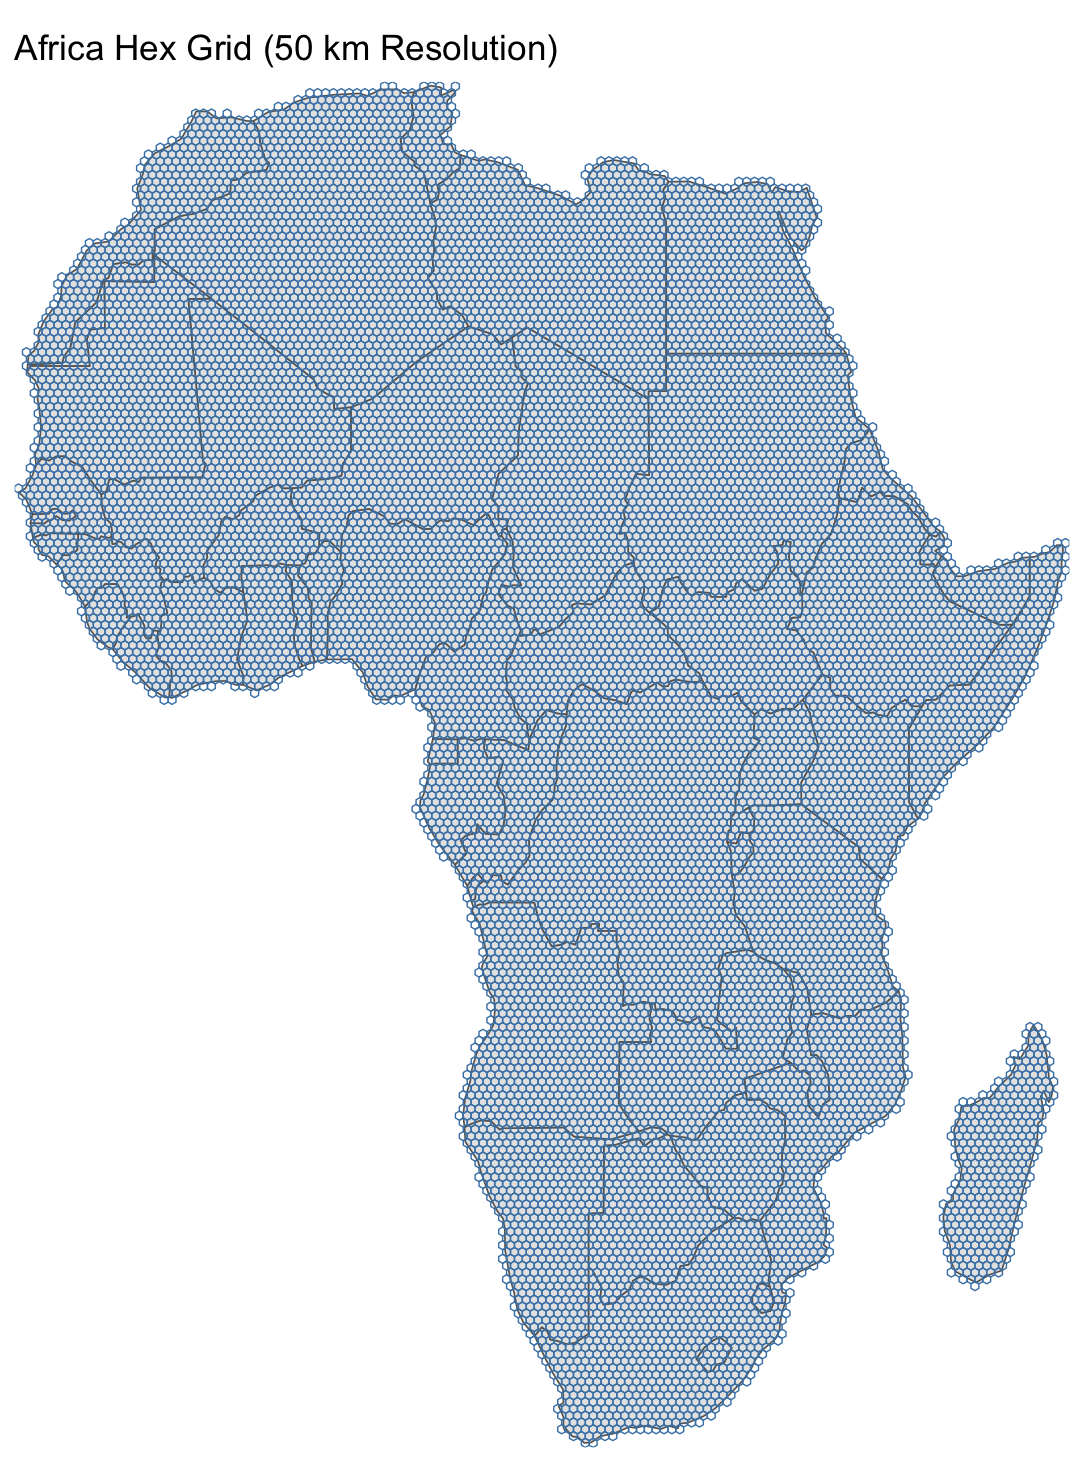
\includegraphics[width=\textwidth]{plots/Africa50km.png}
{\small\color{muted} 50 km hex grid}

\column{0.39\textwidth}
\centering
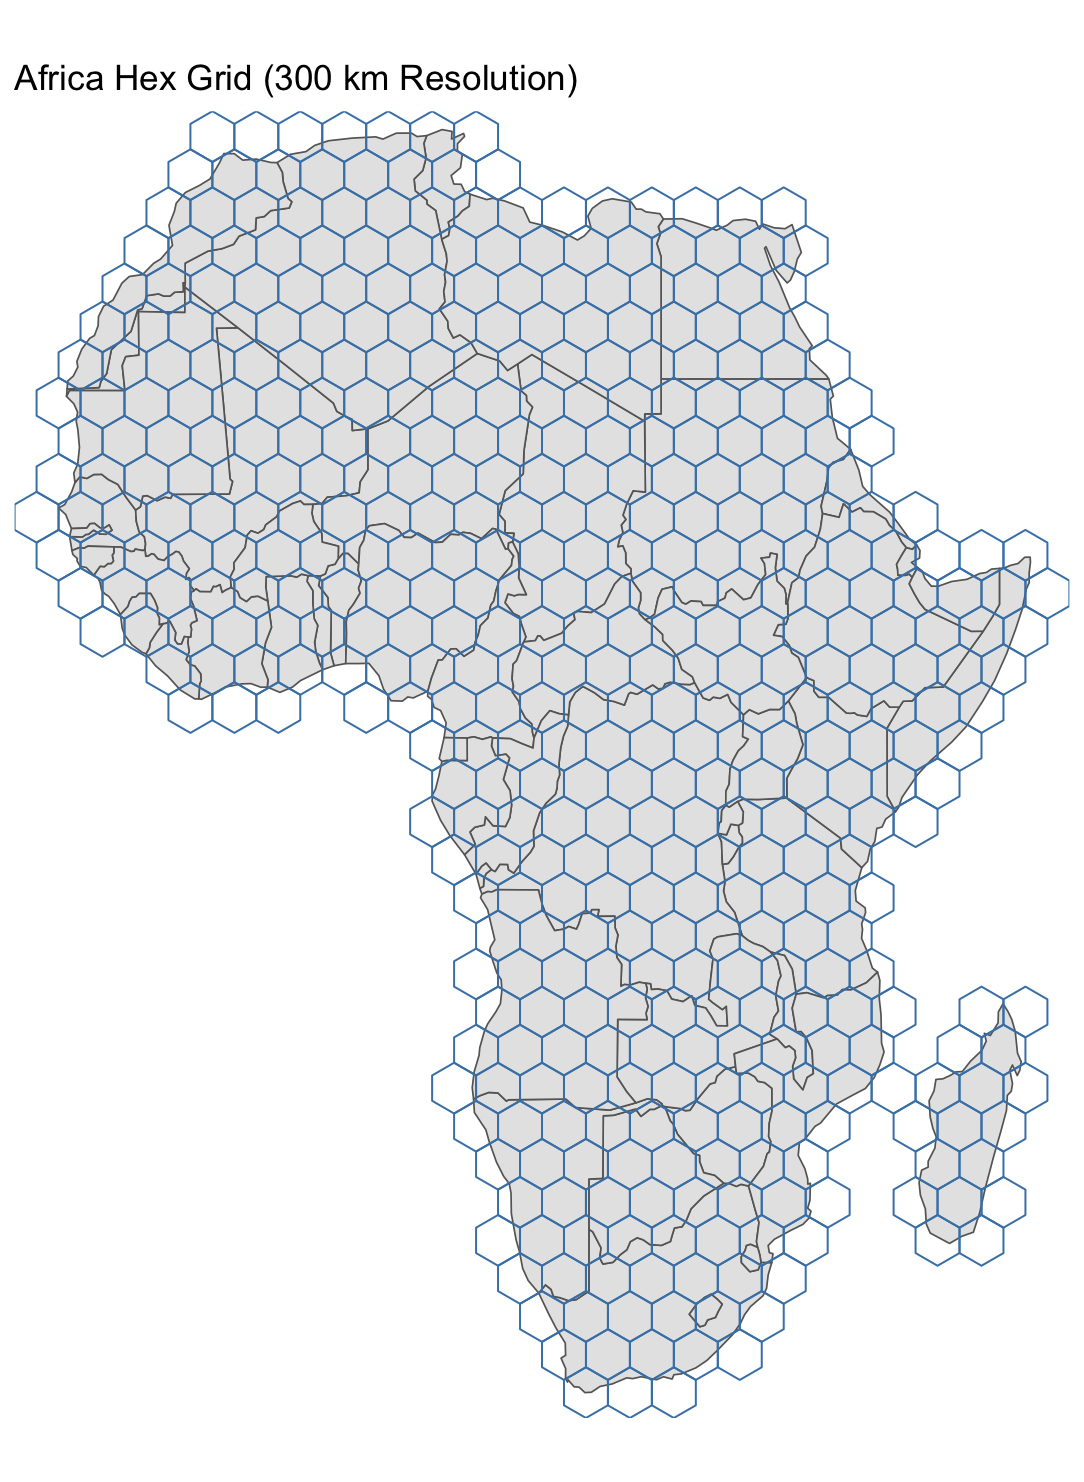
\includegraphics[width=\textwidth]{plots/Africa300km.png}
{\small\color{muted} 300 km hex grid}
\end{columns}

\vspace{0.6em}
{\small Main analysis uses 100km resolution, balancing local precision with sufficient conflict variation. Robustness results are reported across all seven scales (25--300km).}
\end{frame}


\begin{frame}{`Ungoverned' Robustness --- Gallium \& Germanium {\normalsize\color{muted}(Governance Gap)}}
{\footnotesize Cells report number of significant post-treatment periods ($p<0.05$), direction in parentheses.}

\vspace{0.3em}
{\footnotesize
\begin{tabular}{lccccc}
\toprule
\textcolor{lime}{\textbf{Scale}} & \textcolor{lime}{\textbf{All Events}} & \textcolor{lime}{\textbf{Battle Deaths}} & \textcolor{lime}{\textbf{State-Based}} & \textcolor{lime}{\textbf{Non-State}} & \textcolor{lime}{\textbf{One-Sided}} \\
\midrule
300km & 3 (Neg) & ---     & ---      & 3 (Neg) & ---     \\
250km & 4 (Neg) & 5 (Pos) & ---      & 3 (Neg) & ---     \\
200km & 4 (Neg) & 4 (Pos) & 3 (Neg)  & 3 (Neg) & 4 (Neg) \\
150km & 4 (Neg) & 3 (Pos) & 5 (Neg)  & 3 (Neg) & 5 (Neg) \\
100km & 5 (Neg) & 5 (Pos) & 6 (Neg)  & 3 (Neg) & 6 (Neg) \\
050km & 9 (Neg) & 5 (Pos) & 9 (Neg)  & 7 (Neg) & 7 (Neg) \\
025km & 9 (Neg) & 6 (Pos) & 10 (Neg) & 7 (Neg) & 9 (Neg) \\
\bottomrule
\end{tabular}
}

\vspace{0.4em}
{\small\color{lime} Decoupling strengthens at finer scales: 3 significant event-reduction periods at 300km vs.\ 9 at 25km. Battle death increases only emerge below 250km, consistent with localised competition at ungoverned sites.}
\end{frame}



% ═══════════════════════════════════════════════
% DISCUSSION AND QuestionS
% ═══════════════════════════════════════════════

\begin{frame}{What This Suggests}
\begin{itemize}
    \item `Green' mineral wealth does not \textit{mechanically} produce conflict. Governance mediates the relationship.
    \item But governance gaps create new risks. The decoupling pattern for Ga/Ge could foreshadow new ``blood minerals'' as the energy transition accelerates.
\end{itemize}
\end{frame}

\begin{frame}{Question 1: Discovery vs.\ Mining}
Our identification uses mineral \textbf{discovery} (not production) as treatment.

\vspace{0.5em}
\textcolor{sage}{\textbf{Advantages:}}
\begin{itemize}
    \item Discovery timing is plausibly exogenous to local conflict.
    \item Captures anticipatory effects before extraction begins.
\end{itemize}

\vspace{0.3em}
\textcolor{lime}{\textbf{Limitations:}}
\begin{itemize}
    \item Mining generates actual revenue flows, employment, infrastructure.
    \item The ``development'' channel could amplify or reverse discovery effects.
\end{itemize}

\vspace{0.5em}
\audience{Should we extend the analysis to mine openings and production? Or is the discovery design enough for a first paper?}
\end{frame}

\begin{frame}{Question 2: The Cobalt Problem}
Cobalt is arguably the most important critical mineral for the energy transition. But we excluded it due to \textbf{messy pre--trends}.

\vspace{0.5em}
\textcolor{lime}{\textbf{The challenge:}}
\begin{itemize}
    \item Most cobalt comes from the DRC, which has sustained conflict predating mineral discovery.
    \item Parallel trends assumption is hard to satisfy.
    \item Possible approaches: DRC--specific analysis, excluding DRC, sub--national controls.
\end{itemize}

\vspace{0.5em}
\audience{Is the paper complete without cobalt? Or is it too conspicuous an omission?}
\end{frame}


\begin{frame}{Question 3: Which Type of Violence?}
We present non--state violence because it is the most robust outcome. But we have results for all types.

\vspace{0.5em}
\textcolor{sage}{\textbf{Available outcomes:}}
\begin{itemize}
    \item \textbf{Non--state violence} (armed groups vs.\ armed groups): most directly tied to contestation over mineral rents.
    \item \textbf{State--based violence} (government vs.\ opposition): may respond differently if governance strengthens state presence at extraction sites.
    \item \textbf{One--sided violence} (against civilians): could increase even as inter--group conflict falls, if armed actors shift tactics.
\end{itemize}

\vspace{0.3em}

\audience{Is non--state violence the right headline outcome? Or should we build distinct predictions for each violence type into the framework?}
\end{frame}


\begin{frame}{Question 4: Strengthening the Framework}
The three--tier governance framework is the paper's main conceptual contribution. But it is currently underdeveloped.

\vspace{0.5em}
\textcolor{sage}{\textbf{Areas to develop:}}
\begin{itemize}
    \item Formalising the mechanisms behind each pathway.
    \item Addressing alternative explanations (geology vs.\ governance, spatial displacement, peacekeeping confounds).
\end{itemize}

\vspace{0.5em}
\audience{Is this governance thing a sufficient analytical framework?}
\end{frame}

\begin{frame}{What Else Is Needed?}
\textcolor{sage}{\textbf{Possible extensions we are considering:}}
\begin{itemize}
    \item Heterogeneity by country--level institutions (state capacity, rule of law).
    \item We have this data for both Africa and Asia...
    \item Is this a story about governance at all?
    \item How much to frame around 'green' resources (also important for military)?
           \begin{itemize}
             
           \item Is this a story about industry demand (e.g. Ga/Ge used in radar/military - the least `green')? 
\end{itemize} 
    \item Should we compare state vs. non-state violence?
\end{itemize}

\vspace{0.5em}
\audience{Which extensions matter most for a first paper? Where should this land (Conflict, Political Science, Environmental, Science/short form)?}
\end{frame}

\begin{frame}
\begin{center}
\vspace{2em}
{\Large\color{cream}\textbf{Thank you!}}

\vspace{1.5em}
{\normalsize\color{sage} Elisa D'Amico \quad $\cdot$ \quad elisa.damico@ucd.ie}

\vspace{0.3em}
{\normalsize\color{lime} P\"aivi Lujala \quad $\cdot$ \quad paivi.lujala@oulu.fi}
\end{center}
\end{frame}

\appendix



\begin{frame}{Appendix: Scale Robustness --- Tantalum \& Tin {\normalsize\color{muted}(3T Governed)}}
{\footnotesize Cells report number of significant post-treatment periods ($p<0.05$), direction in parentheses. ``---'' = no significant effects.}

\vspace{0.3em}
{\footnotesize
\begin{tabular}{lcccc}
\toprule
\textcolor{sage}{\textbf{Scale}} & \textcolor{sage}{\textbf{All Events}} & \textcolor{sage}{\textbf{Battle Deaths}} & \textcolor{sage}{\textbf{Non-State}} & \textcolor{sage}{\textbf{One-Sided}} \\
\midrule
\multicolumn{5}{l}{\textit{Tantalum}} \\
300km & 7 (Neg) & ---     & ---      & ---      \\
250km & ---     & ---     & 20 (Neg) & ---      \\
150km & ---     & ---     & ---      & 9 (Neg)  \\
100km & ---     & 9 (Neg) & ---      & 7 (Neg)  \\
050km & ---     & ---     & 5 (Neg)  & ---      \\
\midrule
\multicolumn{5}{l}{\textit{Tin}} \\
300km & ---     & ---     & 4 (Neg)  & ---      \\
250km & ---     & ---     & 20 (Neg) & ---      \\
200km & ---     & ---     & 20 (Neg) & ---      \\
150km & ---     & ---     & 5 (Neg)  & ---      \\
\bottomrule
\end{tabular}
}

\vspace{0.4em}
{\small\color{sage} Neither mineral shows increased battle deaths at any scale. Strongest effects at coarser resolutions, consistent with regional supply chain mechanisms.}
\end{frame}

\begin{frame}{Appendix: Scale Robustness --- Platinum Group Metals {\normalsize\color{muted}(Nationally Governed)}}
{\footnotesize Cells report number of significant post-treatment periods ($p<0.05$), direction in parentheses.}

\vspace{0.3em}
{\footnotesize
\begin{tabular}{lccccc}
\toprule
\textcolor{muted}{\textbf{Scale}} & \textcolor{muted}{\textbf{All Events}} & \textcolor{muted}{\textbf{Battle Deaths}} & \textcolor{muted}{\textbf{State-Based}} & \textcolor{muted}{\textbf{Non-State}} & \textcolor{muted}{\textbf{One-Sided}} \\
\midrule
300km & ---     & ---     & ---     & 8 (Neg)  & --- \\
250km & 3 (Neg) & ---     & 3 (Neg) & 9 (Neg)  & --- \\
200km & ---     & 7 (Neg) & 7 (Neg) & 10 (Neg) & --- \\
150km & ---     & ---     & ---     & 9 (Neg)  & --- \\
100km & ---     & ---     & ---     & 11 (Neg) & --- \\
050km & ---     & ---     & 3 (Neg) & 8 (Neg)  & --- \\
025km & ---     & ---     & 3 (Neg) & 8 (Neg)  & --- \\
\bottomrule
\end{tabular}
}

\vspace{0.4em}
{\small\color{muted} 8--11 significant non-state violence reduction periods at every scale. Spatial stability reflects formal state authority that does not attenuate with distance, unlike market-based or informal mechanisms.}
\end{frame}

\end{document}